
\documentclass[pdf,
%8pt, 9pt, 10pt, 11pt, 12pt, 14pt, 17pt, 20pt
serif,
%handout,	% remove overlays
compress,
xcolor=table,
dvipsnames,
spanish,
aspectratio=169]{beamer}

\usepackage[algosection,lined]{algorithm2e}
\usepackage{minted}
\usepackage{tcolorbox}
\usepackage{xcolor}
\usepackage{comment}
\usepackage{todonotes}
\tcbuselibrary{minted}
\definecolor{bg}{rgb}{0.95,0.95,0.95}

%% Encoding, fonts, language
%\input{settings/pdflatex_setup}
\usepackage{graphics}
\usepackage{url}
\usepackage{amsmath,amssymb,amsfonts,marvosym}
\usepackage{ulem}			% to cross out text
\usepackage{subfig}			% to cross out text
\normalem
\usepackage{ragged2e}
\let\raggedright=\RaggedRight
%\input{settings/beamer_setup}
%\input{settings/biblatex_setup2.tex}

\usepackage{datetime}
\newdateformat{specialdate}{\twodigit{\THEDAY}-\twodigit{\THEMONTH}-\THEYEAR}
%\newdateformat{specialdate}{\twodigit{\THEDAY}-\THEYEAR}
\date{\specialdate\today}

%%%%%%%%%%%%%%%%%%%%%%%%%%%%%%%%%%%%%%%%%%%%%%%%%%%%%%%%%%%%%%%%%
% HEADER
%%%%%%%%%%%%%%%%%%%%%%%%%%%%%%%%%%%%%%%%%%%%%%%%%%%%%%%%%%%%%%%%%

%\title[\arabic{page} ]{Advanced Computer Graphics}
\title[Arrays]{Demo 11: BaseDAtos\_GPS\_SintesisRecVoz-ETC \\for
Jetpack Compose}
% Sin subtitulos
\subtitle[short]{Mobile Programming}
% Corchetes: Solo apellidos de los integrantes, Llaves: Los nombres completos!!
\author[-]{Antonio Isai López Leal}
\institute[UPV]{Polytechnic University of Victoria}
\date[]{September - December 2024}
\logo{\pgfimage[width=1cm,height=1cm]{graphics/logo_upv_transparente}}			% Logo on all slides (pdf,png,jpg,eps)
%\titlegraphic{\includegraphics[height=1.5cm]{graphics/logo_upv_transparente} \hfil \includegraphics[height=1.8cm]{graphics/c++.png}}	% Logo on title slide
\titlegraphic{\includegraphics[height=1.5cm]{graphics/logo_upv_transparente} \hfill  \includegraphics[height=1.5cm]{graphics/kotlin.png}}	% Logo on title slide



%%%%%%%%%%%%%%%%%%%%%%%%%%%%%%%%%%%%%%%%%%%%%%%%%%%%%%%%%%%%%%%%%
% SLIDES
%%%%%%%%%%%%%%%%%%%%%%%%%%%%%%%%%%%%%%%%%%%%%%%%%%%%%%%%%%%%%%%%%

% Configuracion para dibujar AUTOMATAS
\usepackage{tikz}
\usetikzlibrary{shadows,arrows.meta}
\usetikzlibrary{shadows,positioning,arrows}

\tikzset{parent/.style={align=center,text width=2cm,fill=green!20,rounded corners=2pt},
    child/.style={align=center,text width=2.8cm,fill=green!50,rounded corners=6pt},
    grandchild/.style={fill=pink!50,text width=2.3cm}
}
\usetikzlibrary{automata, positioning, arrows}


\begin{document}

\begin{frame}
    \titlepage
\end{frame}

%
\begin{frame}[fragile]
    \frametitle{Abstract}

    \begin{itemize} \item \textbf{Add Tutor:} Inserts a new tutor into the SQLite database, using a name provided by the user. \item \textbf{Delete Tutor:} Removes a tutor by ID. If the ID field is empty, it displays an error message indicating Field is 'empty'. \item \textbf{Update Tutor:} Updates the name of a tutor by ID, modifying the tutor's name if both fields are filled. \item \textbf{View Tutors:} Retrieves a list of all tutors in the format Tutor X: 'Name (ID: Y)' and displays it in a vertical list. \item \textbf{Add Tutored Student:} Associates a 'tutorado' (student) with a specified tutor ID, given both fields are provided. \item \textbf{View Tutored Students by Tutor:} Lists all students associated with a specific tutor ID in a format similar to Tutored Student X: 'Name'. 
    \end{itemize}
    
\end{frame}
%
\begin{frame}[fragile]
    \frametitle{Original XML Code - activity\_main.xml (1)}    
\begin{columns}
\column{0.65\linewidth}


    \begin{minted}[fontsize=\tiny]{xml}
ScrollView
    xmlns:android="http://schemas.android.com/apk/res/android"
    xmlns:tools="http://schemas.android.com/tools"
    android:layout_width="match_parent"
    android:layout_height="match_parent"
    android:orientation="vertical"  
    >
    
<LinearLayout 
    android:layout_width="match_parent"
    android:layout_height="match_parent"
    android:orientation="vertical"
    tools:context=".MainActivity" >
    <TextView	            
        android:layout_height="wrap_content"
        android:layout_width="fill_parent"
        android:id="@+id/TV4"
        android:text="NOMBRE DEL TUTOR" />
    <EditText
        android:id="@+id/ET2"        
        android:layout_width="fill_parent"
        android:layout_height="wrap_content"
        android:text="" />
    <TextView
        android:layout_height="wrap_content"
        android:layout_width="fill_parent"
        android:id="@+id/TV5"
        android:text="ID TUTOR ACTUALIZAR/MODIFICAR" />
    \end{minted}
\column{0.35\linewidth}
\begin{itemize}\tiny
        \item The layout starts with a \texttt{ScrollView} to enable vertical scrolling, containing a vertically oriented \texttt{LinearLayout}.
        \item At the top, there is a \texttt{TextView} labeled \emph{NOMBRE DEL TUTOR} followed by an \texttt{EditText} (ID: \texttt{ET2}) for entering the tutor's name.
        \item Another \texttt{TextView} labeled \emph{ID TUTOR ACTUALIZAR/MODIFICAR} indicates the input field for tutor ID.
    \end{itemize}
\end{columns}  
\end{frame}
%%%%%%%%%%%%%%%%%%%%%%%%%%%%%%%%%
\begin{frame}[fragile]
    \frametitle{Original XML Code - activity\_main.xml (2)}    


\begin{columns}
\column{0.65\linewidth}
    \begin{minted}[fontsize=\tiny]{xml}


    <EditText    
        android:id="@+id/ET1"        
        android:layout_width="fill_parent"
        android:layout_height="wrap_content"
        android:text="" />
    <TextView
        android:layout_height="wrap_content"
        android:layout_width="fill_parent"
        android:id="@+id/TV6"
        android:text="Nombre del Tutorado" />
     <EditText
        android:id="@+id/ET3"
        android:layout_width="fill_parent"
        android:layout_height="wrap_content"
        android:text="0" />
	        <Button
	            android:layout_width="fill_parent"
	            android:layout_height="fill_parent"
	            android:text="Insertar Tutor"
	            android:id="@+id/BT01"   />
	        <Button
	            android:layout_width="fill_parent"
	            android:layout_height="fill_parent"
	            android:text="Borrar Tutor"
	            android:id="@+id/BT02"   />	        	        
	        

    \end{minted}
\column{0.35\linewidth}
\begin{itemize}\tiny
        \item An \texttt{EditText} (ID: \texttt{ET1}) is placed next to accept the tutor's ID, followed by a \texttt{TextView} labeled \emph{Nombre del Tutorado}.
        \item Another \texttt{EditText} (ID: \texttt{ET3}) is provided below to enter the tutored person's name.
        \item This section is followed by a series of buttons for different actions, starting with \emph{Insertar Tutor} (ID: \texttt{BT01}) and \emph{Borrar Tutor} (ID: \texttt{BT02}).
    \end{itemize}
\end{columns}  
\end{frame}
%%%%%%%%%%%%%%%%%%%%%%%%%%%%%%%%%%5
\begin{frame}[fragile]
    \frametitle{Original XML Code - activity\_main.xml (3)}    


\begin{columns}
\column{0.65\linewidth}
    \begin{minted}[fontsize=\tiny]{xml}
     <Button
	            android:layout_width="fill_parent"
	            android:layout_height="fill_parent"
	            android:text="Consultar Tutores"
	            android:id="@+id/BT03"   />	        	        
	        <Button
	            android:layout_width="fill_parent"
	            android:layout_height="fill_parent"
	            android:text="Actualizar Tutor"
	            android:id="@+id/BT04"   />
	        <Button
	            android:layout_width="fill_parent"
	            android:layout_height="fill_parent"
	            android:text="Agregar Tutorado"
	            android:id="@+id/BT05"   />	        	        
	        <Button
	            android:layout_width="fill_parent"
	            android:layout_height="fill_parent"
	            android:text="Consultar Tutorados por Tutor"
	            android:id="@+id/BT06"   />
	<Button
		android:layout_width="fill_parent"
		android:layout_height="fill_parent"
		android:text="Otra ACtividad"
		android:id="@+id/BT07"   />
	<TextView
        android:layout_height="wrap_content"
        android:layout_width="fill_parent"
        android:id="@+id/TV2"
        android:text="CONTENIDO DEL TEXTIVIEW" />        
</LinearLayout>
</ScrollView>

    \end{minted}
\column{0.35\linewidth}
\begin{itemize}\tiny
        \item Additional buttons allow for further actions like \emph{Consultar Tutores}, \emph{Actualizar Tutor}, and more, each with a unique ID (e.g., \texttt{BT03}, \texttt{BT04}).
        \item At the bottom, a \texttt{TextView} (ID: \texttt{TV2}) displays the content or results of operations.
    \end{itemize}
\end{columns}  
\end{frame}

%%%%%%%%%%%%%%%%%%%%%%%%%%%%%%%%%%%%%%%%%%%%%%%%

\begin{frame}[fragile]
    \frametitle{Original XML Code - activity\_main2.xml}    
\begin{columns}
\column{0.65\linewidth}
    \begin{minted}[fontsize=\tiny]{xml}
<ScrollView
    xmlns:android="http://schemas.android.com/apk/res/android"
    xmlns:tools="http://schemas.android.com/tools"
    android:layout_width="match_parent"
    android:layout_height="match_parent"
    android:orientation="vertical"
    >

<LinearLayout 
    
    android:layout_width="match_parent"
    android:layout_height="match_parent"
    android:orientation="vertical"
    tools:context=".MainActivity" >
    
	        <Button
	            android:layout_width="fill_parent"
	            android:layout_height="fill_parent"
	            android:text="Insertar Tutor"
	            android:id="@+id/BT01_AC2"   />
	<TextView
		android:id="@+id/TV_MARCIANO1"
		android:layout_width="match_parent"
		android:layout_height="match_parent" />
</LinearLayout>
</ScrollView>

    \end{minted}
\column{0.35\linewidth}
\begin{itemize}\tiny
\item The layout is structured to make interactions intuitive, with each button handling a specific operation.
\end{itemize}
\end{columns}  
\end{frame}

%%%%%%%%%%%%%%%%%%%%%%%%%%%%%%

\begin{frame}
\frametitle{Composable Functions and Compose Modifiers in Android}
\begin{columns}
\column{0.45\linewidth}
\textbf{Composable Functions:}
\begin{itemize}\tiny
    \item A Composable function is a modern way to build UI in Android, written directly in Kotlin. 
    \item It is annotated with \texttt{@Composable}, which signals to the Compose compiler that the function is for UI construction.
    \item Unlike traditional XML layouts, Composable functions allow for a more flexible, programmatic approach to UI development.
    \item In our project, \texttt{TutorScreen}, \texttt{ActionButton}, and various UI elements like \texttt{TextField} are implemented as Composable functions.
\end{itemize}

\column{0.45\linewidth}
\textbf{Compose Modifiers:} 
\begin{itemize}\tiny
    \item Compose modifiers allow you to decorate or enhance a Composable, controlling its size, layout, and behavior.
    \item For example, in our project, we use \texttt{Modifier.fillMaxWidth()} and \texttt{Modifier.padding()} to adjust the width and padding of UI elements.
    \item Modifiers can also handle interactions, making elements clickable, scrollable, or draggable.
    \item They allow us to enrich the UI with functionalities like accessibility labels and processing user input.
\end{itemize}
\end{columns}
\end{frame}

%%%%%%%%%%%%%%%%%%%%%%%%%%%%%%%%%%%%%%%%%%%%%%%%%%%%%%%%%

\begin{frame}[fragile]
    \frametitle{Main Activity of a Kotlin App using Composables}
\begin{minted}[fontsize=\tiny]{Kotlin}
class MainActivity : ComponentActivity() {
    private lateinit var databaseHelper: TutorDatabaseHelper

    override fun onCreate(savedInstanceState: Bundle?) {
        super.onCreate(savedInstanceState)
        databaseHelper = TutorDatabaseHelper(this)
        setContent {
            TutorScreen(databaseHelper)
        }
    }
}
\end{minted}
\end{frame}

%%%%%%%%%%%%%%%%%%%%%%%%%%%%%%%%%%

\begin{frame}[fragile]
    \frametitle{MainScreen Composable (1) - MainActivity.kt}
\begin{columns}
\column{0.55\linewidth}
\begin{minted}[fontsize=\tiny]{Kotlin}

package com.z_iti_271311_u1_ae_lopez_leal_antonio_isai

import android.os.Bundle
import androidx.activity.ComponentActivity
import androidx.activity.compose.setContent
import androidx.compose.foundation.layout.*
import androidx.compose.foundation.lazy.LazyColumn
import androidx.compose.foundation.lazy.items
import androidx.compose.material3.Button
import androidx.compose.material3.Text
import androidx.compose.material3.TextField
import androidx.compose.runtime.*
import androidx.compose.ui.Alignment
import androidx.compose.ui.Modifier
import androidx.compose.ui.text.input.TextFieldValue
import androidx.compose.ui.unit.dp
import com.z_iti_271311_u1_ae_lopez_leal_antonio_isai.data.TutorDatabaseHelper

\end{minted}
\column{0.45\linewidth}

\begin{itemize}\tiny
    \item Create a new project in Android Studio using "Empty Compose Activity" as the template.
    
    \item In the \texttt{kotlin+java} directory, create a new package named \texttt{data} to organize database-related files.
    \item Inside the \texttt{data} package, add a file named \texttt{TutorDatabaseHelper.kt} to define database operations for managing tutors and students.
    \item Open \texttt{MainActivity.kt} and replace its content with the main UI and logic setup to enable CRUD operations and display results.
\end{itemize}

\end{columns}
\end{frame}

%%%%%%%%%%%%%%%%%%%%%%%%%%%%%%%%%%

\begin{frame}[fragile]
    \frametitle{MainScreen Composable (2) - MainActivity.kt}
\begin{columns}
\column{0.55\linewidth}
\begin{minted}[fontsize=\tiny]{Kotlin}
@Composable
fun TutorScreen(databaseHelper: TutorDatabaseHelper) {
    val tutorName = remember { mutableStateOf(TextFieldValue()) }
    val tutorId = remember { mutableStateOf(TextFieldValue()) }
    val tutoredName = remember { mutableStateOf(TextFieldValue("0")) }
    
    var resultList by remember { mutableStateOf(listOf<String>()) }

    Column(
        modifier = Modifier
            .fillMaxSize()
            .padding(16.dp),
        horizontalAlignment = Alignment.CenterHorizontally
    ) {
        
        TextField(
            value = tutorName.value,
            onValueChange = { tutorName.value = it },
            label = { Text("Nombre del Tutor") },
            modifier = Modifier.fillMaxWidth()
        )
        Spacer(modifier = Modifier.height(8.dp))

        TextField(
            value = tutorId.value,
            onValueChange = { tutorId.value = it },
            label = { Text("ID Tutor Actualizar/Modificar") },
            modifier = Modifier.fillMaxWidth()
        )
        Spacer(modifier = Modifier.height(8.dp))
        
\end{minted}
\column{0.45\linewidth}
\begin{itemize}\tiny
    \item \textbf{@Composable fun TutorScreen(databaseHelper: TutorDatabaseHelper)} - A composable function that displays a screen for managing tutors and students (tutorados) with a provided \texttt{databaseHelper} object for database operations. It includes input fields and a list to display results from database actions.
    
    \item \textbf{State Variables:}
    \begin{itemize}\tiny
        \item \texttt{tutorName}: A mutable state holding the name of the tutor entered by the user. Initialized as an empty \texttt{TextFieldValue}.
        \item \texttt{tutorId}: A mutable state for the tutor’s ID, used for updating or deleting records. Also initialized as an empty \texttt{TextFieldValue}.
        \item \texttt{tutoredName}: Holds the name of the student (tutorado) associated with a tutor, initialized with the default value of \texttt{"0"}.
        \item \texttt{resultList}: A mutable state containing the list of strings used to display the result of database operations (e.g., successful insertion or deletion).
    \end{itemize}

    
\end{itemize}
\end{columns}
\end{frame}

%%%%%%%%%%%%%%%%%%%%%%%%%%%%%%%%%%

\begin{frame}[fragile]
    \frametitle{MainScreen Composable (3) - MainActivity.kt}
\begin{columns}
\column{0.55\linewidth}
\begin{minted}[fontsize=\tiny]{Kotlin}
TextField(
            value = tutoredName.value,
            onValueChange = { tutoredName.value = it },
            label = { Text("Nombre del Tutorado") },
            modifier = Modifier.fillMaxWidth()
        )
        Spacer(modifier = Modifier.height(16.dp))
       
        ActionButton("INSERTAR TUTOR") {
            if (tutorName.value.text.isEmpty()) {
                resultList = listOf("CAMPO VACÍO: 
                Por favor ingresa el nombre del tutor.")
            } else {
                databaseHelper.insertTutor(tutorName.value.text)
                resultList = listOf("Tutor 
                '${tutorName.value.text}' insertado.")
            }
        }
        ActionButton("BORRAR TUTOR") {
            if (tutorId.value.text.isEmpty()) {
                resultList = listOf("CAMPO VACÍO: Por favor ingresa el ID del tutor.")
            } else {
                databaseHelper.deleteTutor(tutorId.value.text.toLong())
                resultList = listOf("Tutor con ID ${tutorId.value.text} eliminado.")
            }
        }
\end{minted}
\column{0.45\linewidth}
\item \tiny \textbf{UI Structure with Column:}
    \begin{itemize}\tiny
        \item Uses \texttt{Column} to organize composables vertically, filling the screen’s size with \texttt{Modifier.fillMaxSize()} and adding padding.
        \item Aligns all child composables horizontally at the center with \texttt{horizontalAlignment = Alignment.CenterHorizontally}.
    \end{itemize}
\end{columns}
\end{frame}

%%%%%%%%%%%%%%%%%%%%%%%%%%%%%%%%%%

\begin{frame}[fragile]
    \frametitle{MainScreen Composable (4) - MainActivity.kt}
\begin{columns}
\column{0.55\linewidth}
\begin{minted}[fontsize=\tiny]{Kotlin}
ActionButton("CONSULTAR TUTORES") {
            val tutors = databaseHelper.getTutors()
            if (tutors.isEmpty()) {
                resultList = listOf("No hay tutores para mostrar.")
            } else {
                resultList = tutors.mapIndexed { index, (id, name) -> "Tutor ${index + 1}: $name (ID: $id)" }
            }
        }
        ActionButton("ACTUALIZAR TUTOR") {
            if (tutorId.value.text.isEmpty()
            || tutorName.value.text.isEmpty()) {
                resultList = listOf("CAMPO VACÍO: 
                Por favor ingresa el ID y 
                el nombre del tutor.")
            } else {
                databaseHelper.updateTutor
                (tutorId.value.text.toLong(),tutorName.value.text)
                resultList = listOf("Tutor con ID ${tutorId.value.text} 
                actualizado a '${tutorName.value.text}'.")
            }
        }
        ActionButton("AGREGAR TUTORADO") {
            if (tutoredName.value.text.isEmpty() || tutorId.value.text.isEmpty()) {
                resultList = listOf("CAMPO VACÍO: Por favor ingresa el nombre del tutorado y el ID del tutor.")
            } else {
                databaseHelper.addTutorado(tutoredName.value.text, tutorId.value.text.toLong())
                resultList = listOf("Tutorado '${tutoredName.value.text}' agregado al tutor con ID ${tutorId.value.text}.")
            }
        }
\end{minted}
\column{0.45\linewidth}
\item \tiny\textbf{Input Fields:}
    \begin{itemize}\tiny
        \item \texttt{TextField} for \texttt{tutorName}: An input field allowing the user to enter the tutor's name, with a label "Nombre del Tutor" and full width.
        \item \texttt{TextField} for \texttt{tutorId}: Another input field where the user enters the tutor’s ID for modification or deletion purposes, labeled "ID Tutor Actualizar/Modificar".
        \item Adds \texttt{Spacer} elements between fields to add vertical spacing.
    \end{itemize}
\end{columns}
\end{frame}

%%%%%%%%%%%%%%%%%%%%%%%%%%%%%%%%%%

\begin{frame}[fragile]
    \frametitle{MainScreen Composable (5) - MainActivity.kt}
\begin{columns}
\column{0.55\linewidth}
\begin{minted}[fontsize=\tiny]{Kotlin}
ActionButton("CONSULTAR TUTORADOS POR TUTOR") {
            if (tutorId.value.text.isEmpty()) {
                resultList = listOf("CAMPO VACÍO: Por favor ingresa el ID del tutor.")
            } else {
                val tutorados = databaseHelper.getTutoradosByTutor(tutorId.value.text.toLong())
                if (tutorados.isEmpty()) {
                    resultList = listOf("No hay tutorados para el tutor con ID ${tutorId.value.text}.")
                } else {
                    resultList = tutorados.mapIndexed { index, tutorado -> "Tutorado ${index + 1}: $tutorado" }
                }
            }
        }
        Spacer(modifier = Modifier.height(16.dp))
        
        LazyColumn(
            modifier = Modifier
                .fillMaxWidth()
                .padding(16.dp)
        ) {
            items(resultList) { item ->
                Text(text = item, modifier = Modifier.padding(vertical = 4.dp))
            }
        }
    }
}
\end{minted}
\column{0.45\linewidth}
\end{columns}
\end{frame}

%%%%%%%%%%%%%%%%%%%%%%%%%%%%%%%%%%

\begin{frame}[fragile]
    \frametitle{MainScreen Composable (6) - MainActivity.kt}
\begin{columns}
\column{0.45\linewidth}
\begin{minted}[fontsize=\tiny]{Kotlin}
@Composable
fun ActionButton(text: String, onClick: () -> Unit) {
    Button(
        onClick = onClick,
        modifier = Modifier
            .fillMaxWidth()
            .padding(vertical = 4.dp)
    ) {
        Text(text)
    }
}
\end{minted}
\column{0.45\linewidth}\begin{itemize}
    \item\tiny \textbf{@Composable fun ActionButton(text: String, onClick: () -> Unit)} - A reusable composable function that creates a button with customizable text and action. The button is styled to occupy the full width of its container with vertical padding for spacing.

    \item\tiny  \textbf{Parameters:}
    \begin{itemize}\tiny 
        \item \texttt{text}: A \texttt{String} parameter that defines the label displayed on the button.
        \item \texttt{onClick}: A lambda function (\texttt{() -> Unit}) that specifies the action to perform when the button is clicked.
    \end{itemize}

    \item\tiny  \textbf{Button Component:}
    \begin{itemize}\tiny 
        \item \texttt{Button}: The main clickable component. It triggers the \texttt{onClick} action passed as a parameter.
        \item \texttt{modifier = Modifier.fillMaxWidth()}: Ensures the button spans the entire width of its parent container.
        \item \texttt{modifier.padding(vertical = 4.dp)}: Adds vertical padding (4.dp) above and below the button for spacing.
    \end{itemize}

    \item \tiny \textbf{Text Component:}
    \begin{itemize}\tiny 
        \item Displays the \texttt{text} parameter as the button's label.
    \end{itemize}
\end{itemize}

\end{columns}
\end{frame}
%%%%%%%%%%%%%%%%%%%%%%%%%%%%%%%%%%

\begin{frame}[fragile]
    \frametitle{Component Hierarchy}
 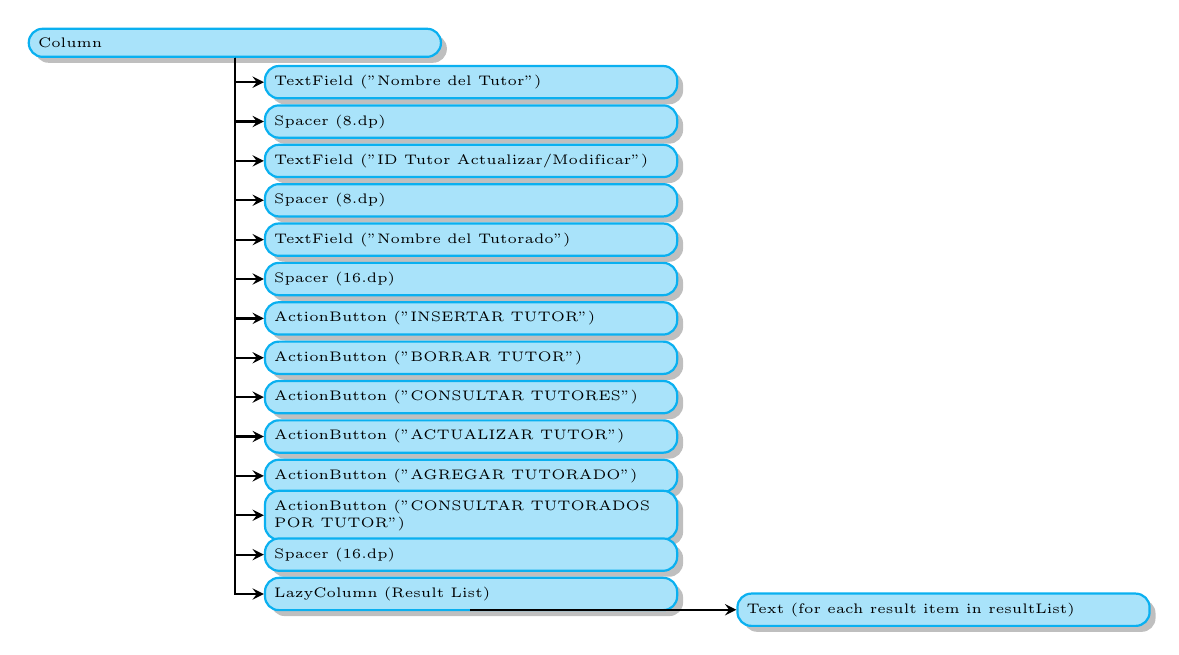
\begin{tikzpicture}[
text width=5cm,
ar/.style={->,>=stealth,thick},
every node/.style={rectangle,rounded corners=5pt,drop shadow,draw=ProcessBlue,fill=ProcessBlue!35,thick, font=\tiny}]
    \node (n0) {Column};
    \node (n1) at (0,-.5) [xshift=3cm] {TextField ("Nombre del Tutor")};
    \node (n2) at (0,-1.0) [xshift=3cm] {Spacer (8.dp)};
    \node (n3) at (0,-1.5) [xshift=3cm] {TextField ("ID Tutor Actualizar/Modificar")};
    \node (n4) at (0,-2.0) [xshift=3cm] {Spacer (8.dp)};
    \node (n5) at (0,-2.5) [xshift=3cm] {TextField ("Nombre del Tutorado")};
    \node (n6) at (0,-3.0) [xshift=3cm] {Spacer (16.dp)};
    \node (n7) at (0,-3.5) [xshift=3cm] {ActionButton ("INSERTAR TUTOR")};
    \node (n8) at (0,-4.0) [xshift=3cm] {ActionButton ("BORRAR TUTOR")};
    \node (n9) at (0,-4.5) [xshift=3cm] {ActionButton ("CONSULTAR TUTORES")};
    \node (n10) at (0,-5) [xshift=3cm] {ActionButton ("ACTUALIZAR TUTOR")};
    \node (n11) at (0,-5.5) [xshift=3cm] {ActionButton ("AGREGAR TUTORADO")};
    \node (n12) at (0,-6) [xshift=3cm] {ActionButton ("CONSULTAR TUTORADOS POR TUTOR")};
    \node (n13) at (0,-6.5) [xshift=3cm] {Spacer (16.dp)};
    \node (n14) at (0,-7) [xshift=3cm] {LazyColumn (Result List)};
    \node (n15) at (6,-7.2) [xshift=3cm] {Text (for each result item in resultList)};
    %\node (n4) at (0,-6) [xshift=6cm] {long text \\overflowing the shape};
    %\node (n5) at (0,-7.5) [xshift=6cm] {long text \\overflowing the shape};
    % Conecta Nodo 0=>1, 0=>2, 0=>3, 3=>4 y 3=>5
    %\foreach \ns/\ne in{0/1,0/2,0/3,3/4,3/5}
    \foreach \ns/\ne in{0/1,0/2,0/3,0/4,0/5,0/6,0/7,0/8,0/9,0/10,0/11,0/12,0/13,0/14,14/15}
    \draw[ar] (n\ns) |- (n\ne);
    
    \end{tikzpicture}

\end{frame}

%%%%%%%%%%%%%%%%%%%%%%%%%%%%%%%%%%%%%
\begin{frame}
\frametitle{Composable Functions in Android}
\begin{columns}
\column{0.45\linewidth}
Composable Function:
\begin{itemize}\tiny
\item A Composable function is a special type of function in Android used to build UI in a declarative way. It is a Kotlin function annotated with \texttt{@Composable}.
\item The \texttt{@Composable} annotation informs the Compose compiler that the function is meant for UI construction.
\item Unlike traditional XML layouts in Android, Composable functions allow us to create UI using Kotlin code, which is more intuitive and flexible.
\item By annotating a function with \texttt{@Composable}, it becomes a composable function that can be called within other composable functions to build a hierarchy of UI elements.
\end{itemize}
\column{0.45\linewidth}
Compose Modifiers:
\begin{itemize}\tiny
\item Compose Modifiers allow you to decorate or configure composable functions to control their size, layout, behavior, and appearance.
\item Examples of using modifiers include:
    \begin{itemize}\tiny
        \item Setting a composable's size or padding.
        \item Adding interactivity, such as \texttt{clickable}, \texttt{scrollable}, or \texttt{draggable}.
        \item Providing accessibility information, like setting content descriptions.
    \end{itemize}
\item Modifiers are applied in a chain, where each modifier can build upon the previous one, allowing for powerful and flexible customization of composable functions.
\end{itemize}   
\end{columns}
\end{frame}
%%%%%%%%%%%%%%%%%%%%%%%%%%%%%%%%%%%%%%%%%%%%%%%%%
\begin{frame}[fragile]
    \frametitle{TutorDatabaseHelper.kt}
\begin{columns}
\column{0.55\linewidth}
\begin{minted}[fontsize=\tiny]{Kotlin}
import android.content.ContentValues
import android.content.Context
import android.database.sqlite.SQLiteDatabase
import android.database.sqlite.SQLiteOpenHelper

class TutorDatabaseHelper(context: Context) : SQLiteOpenHelper(context, DATABASE_NAME, null, DATABASE_VERSION) {

    override fun onCreate(db: SQLiteDatabase) {
        
        db.execSQL("CREATE TABLE $TABLE_TUTOR (ID INTEGER PRIMARY KEY AUTOINCREMENT, NAME TEXT NOT NULL)")
        
        db.execSQL("CREATE TABLE $TABLE_TUTORADO (ID INTEGER PRIMARY KEY AUTOINCREMENT, " +
                "NAME TEXT NOT NULL, TUTOR_ID INTEGER, FOREIGN KEY (TUTOR_ID) REFERENCES $TABLE_TUTOR(ID))")
    }

    override fun onUpgrade(db: SQLiteDatabase, oldVersion: Int, newVersion: Int) {
        db.execSQL("DROP TABLE IF EXISTS $TABLE_TUTOR")
        db.execSQL("DROP TABLE IF EXISTS $TABLE_TUTORADO")
        onCreate(db)
    }
\end{minted}
\column{0.45\linewidth}
\end{columns}
\end{frame}

%%%%%%%%%%%%%%%%%%%%%%%%%%%%%%%%%%

\begin{frame}[fragile]
    \frametitle{TutorDatabaseHelper.kt}
\begin{columns}
\column{0.55\linewidth}
\begin{minted}[fontsize=\tiny]{Kotlin}

    fun insertTutor(name: String): Long {
        val db = this.writableDatabase
        val values = ContentValues().apply {
            put("NAME", name)
        }
        return db.insert(TABLE_TUTOR, null, values)
    }

    fun deleteTutor(id: Long) {
        val db = this.writableDatabase
        db.delete(TABLE_TUTOR, "ID=?", arrayOf(id.toString()))
    }

    fun updateTutor(id: Long, name: String) {
        val db = this.writableDatabase
        val values = ContentValues().apply {
            put("NAME", name)
        }
        db.update(TABLE_TUTOR, values, "ID=?", arrayOf(id.toString()))
    }

\end{minted}
\column{0.45\linewidth}
\begin{itemize}\tiny
    \item \textbf{insertTutor(name: String): Long} - Inserts a new tutor into the database with the specified name. It creates a \texttt{ContentValues} object containing the tutor's name and inserts it into the \texttt{TABLE\_TUTOR}. Returns the ID of the newly inserted row as a \texttt{Long}.
    
    \item \textbf{deleteTutor(id: Long)} - Deletes a tutor from the database based on the provided ID. It removes the row in \texttt{TABLE\_TUTOR} where the \texttt{ID} matches the specified \texttt{id} parameter.
    
    \item \textbf{updateTutor(id: Long, name: String)} - Updates the name of a tutor in the database based on the provided ID. It creates a \texttt{ContentValues} object with the new name and updates the row in \texttt{TABLE\_TUTOR} where the \texttt{ID} matches the specified \texttt{id} parameter.
\end{itemize}
\end{columns}
\end{frame}

%%%%%%%%%%%%%%%%%%%%%%%%%%%%%%%%%%

\begin{frame}[fragile]
    \frametitle{TutorDatabaseHelper.kt}
\begin{columns}
\column{0.55\linewidth}
\begin{minted}[fontsize=\tiny]{Kotlin}

    fun getTutors(): List<Pair<Long, String>> {
        val db = this.readableDatabase
        val cursor = db.query(TABLE_TUTOR, arrayOf("ID", "NAME"), 
        null, null, null, null, null)
        val tutors = mutableListOf<Pair<Long, String>>()
        while (cursor.moveToNext()) {
            val id = cursor.getLong(cursor.getColumnIndexOrThrow("ID"))
            val name = cursor.getString(cursor.getColumnIndexOrThrow("NAME"))
            tutors.add(Pair(id, name))
        }
        cursor.close()
        return tutors
    }
    
    fun addTutorado(name: String, tutorId: Long): Long {
        val db = this.writableDatabase
        val values = ContentValues().apply {
            put("NAME", name)
            put("TUTOR_ID", tutorId)
        }
        return db.insert(TABLE_TUTORADO, null, values)
    }

\end{minted}
\column{0.45\linewidth}

\begin{itemize}\tiny
    \item \textbf{getTutors(): List<Pair<Long, String>>} - Retrieves a list of all tutors in the database. This function queries \texttt{TABLE\_TUTOR} for the \texttt{ID} and \texttt{NAME} columns and iterates through each row, adding each tutor as a \texttt{Pair} of \texttt{ID} and \texttt{Name} to a list. The list of tutors is then returned.
    
    \item \textbf{addTutorado(name: String, tutorId: Long): Long} - Adds a new student (tutorado) associated with a specific tutor to the database. It creates a \texttt{ContentValues} object containing the student's \texttt{name} and the \texttt{tutorId} of the associated tutor, then inserts this data into \texttt{TABLE\_TUTORADO}. Returns the ID of the newly inserted row as a \texttt{Long}.
\end{itemize}


\end{columns}
\end{frame}

%%%%%%%%%%%%%%%%%%%%%%%%%%%%%%%%%%

\begin{frame}[fragile]
    \frametitle{TutorDatabaseHelper.kt}
\begin{columns}
\column{0.55\linewidth}
\begin{minted}[fontsize=\tiny]{Kotlin}

    fun getTutoradosByTutor(tutorId: Long): List<String> {
        val db = this.readableDatabase
        val cursor = db.query(TABLE_TUTORADO, arrayOf("ID", "NAME")
        , "TUTOR_ID=?", arrayOf(tutorId.toString()), 
        null, null, null)
        val tutorados = mutableListOf<String>()
        while (cursor.moveToNext()) {
            val name = cursor.getString(cursor.getColumnIndexOrThrow("NAME"))
            tutorados.add(name)
        }
        cursor.close()
        return tutorados
    }

    companion object {
        private const val DATABASE_VERSION = 1
        private const val DATABASE_NAME = "tutorDB"
        const val TABLE_TUTOR = "Tutor"
        const val TABLE_TUTORADO = "Tutorado"
    }
}

\end{minted}
\column{0.45\linewidth}
\begin{itemize}\tiny
    \item \textbf{getTutoradosByTutor(tutorId: Long): List<String>} - Retrieves a list of students (\texttt{tutorados}) associated with a specific tutor based on the provided \texttt{tutorId}. This function queries \texttt{TABLE\_TUTORADO} for entries where \texttt{TUTOR\_ID} matches the specified \texttt{tutorId} and retrieves the \texttt{NAME} of each student. It adds each name to a list, which is returned as the result.

    \item \textbf{companion object} - Defines constants and database configuration for \texttt{TutorDatabaseHelper}:
    \begin{itemize}\tiny
        \item \texttt{DATABASE\_VERSION}: The version of the database, set to \texttt{1}.
        \item \texttt{DATABASE\_NAME}: The name of the database, defined as \texttt{"tutorDB"}.
        \item \texttt{TABLE\_TUTOR}: The name of the table storing tutor information, set as \texttt{"Tutor"}.
        \item \texttt{TABLE\_TUTORADO}: The name of the table storing student information, defined as \texttt{"Tutorado"}.
    \end{itemize}
\end{itemize}

\end{columns}
\end{frame}



%%%%%%%%%%%%%%%%%%%%%%%%%%%%%%%%%%

\begin{frame}[fragile]
    \frametitle{TutorAppTheme.kt}
\begin{columns}
\column{0.55\linewidth}
\begin{minted}[fontsize=\tiny]{Kotlin}
package com.z_iti_271311_u1_ae_lopez_leal_antonio_isai.ui.theme

import androidx.compose.material3.MaterialTheme
import androidx.compose.material3.darkColorScheme
import androidx.compose.material3.lightColorScheme
import androidx.compose.runtime.Composable

private val LightColors = lightColorScheme(
    primary = androidx.compose.ui.graphics.Color(0xFF6200EE),
    onPrimary = androidx.compose.ui.graphics.Color.White,
    secondary = androidx.compose.ui.graphics.Color(0xFF03DAC6),
    onSecondary = androidx.compose.ui.graphics.Color.Black
)

private val DarkColors = darkColorScheme(
    primary = androidx.compose.ui.graphics.Color(0xFFBB86FC),
    onPrimary = androidx.compose.ui.graphics.Color.Black,
    secondary = androidx.compose.ui.graphics.Color(0xFF03DAC6),
    onSecondary = androidx.compose.ui.graphics.Color.Black
)
\end{minted}
\column{0.45\linewidth}

\begin{itemize}\tiny
    \item Create a file named \texttt{TutorAppTheme.kt} in the \texttt{ui.theme} package.
    \item Copy and paste the code provided into \texttt{TutorAppTheme.kt}.
    \item This code defines two color schemes:
    \begin{itemize}\tiny
        \item \texttt{LightColors}: A color scheme for light mode, with primary and secondary colors.
        \item \texttt{DarkColors}: A color scheme for dark mode, with adjusted primary and secondary colors.
    \end{itemize}
    \item These color schemes can be used within \texttt{MaterialTheme} to toggle between light and dark modes.
\end{itemize}


\end{columns}
\end{frame}

%%%%%%%%%%%%%%%%%%%%%%%%%%%%%%%%%%

\begin{frame}[fragile]
    \frametitle{TutorAppTheme.kt}
\begin{columns}
\column{0.55\linewidth}
\begin{minted}[fontsize=\tiny]{Kotlin}
@Composable
fun TutorAppTheme(
    darkTheme: Boolean = false, // Puedes habilitar el tema oscuro si quieres
    content: @Composable () -> Unit
) {
    val colors = if (darkTheme) DarkColors else LightColors

    MaterialTheme(
        colorScheme = colors,
        typography = Typography,
        shapes = Shapes,
        content = content
    )
}
\end{minted}
\column{0.45\linewidth}

\begin{itemize}\tiny
    \begin{itemize}\tiny
        \item \texttt{darkTheme: Boolean = false} - A Boolean parameter that controls whether the dark theme is enabled. By default, it is set to \texttt{false}, meaning the light theme is applied unless specified otherwise.
        \item \texttt{colors} - A variable that selects the appropriate color scheme based on the \texttt{darkTheme} setting. If \texttt{darkTheme} is \texttt{true}, \texttt{DarkColors} is used; otherwise, \texttt{LightColors} is applied.
        \item \texttt{MaterialTheme} - The core theme composable in Jetpack Compose. It applies the selected \texttt{colorScheme}, \texttt{typography}, and \texttt{shapes} to the app's UI components within the provided \texttt{content}.
    \end{itemize}
\end{itemize}

\end{columns}
\end{frame}

%%%%%%%%%%%%%%%%%%%%%%%%%%%%%%%%%%

\begin{frame}[fragile]
    \frametitle{Shapes.kt / Type.kt}
\begin{columns}
\column{0.55\linewidth}
\begin{minted}[fontsize=\tiny]{Kotlin}
// Shapes.kt
package com.z_iti_271311_u1_ae_lopez_leal_antonio_isai.ui.theme

import androidx.compose.material3.Shapes

val Shapes = Shapes()

// Type.kt
package com.z_iti_271311_u1_ae_lopez_leal_antonio_isai.ui.theme

import androidx.compose.material3.Typography
import androidx.compose.ui.text.TextStyle
import androidx.compose.ui.text.font.FontFamily
import androidx.compose.ui.text.font.FontWeight
import androidx.compose.ui.unit.sp

val Typography = Typography(
    bodyLarge = TextStyle(
        fontFamily = FontFamily.Default,
        fontWeight = FontWeight.Normal,
        fontSize = 16.sp,
        lineHeight = 24.sp,
        letterSpacing = 0.5.sp
    )
)
\end{minted}
\column{0.45\linewidth}

\begin{itemize}\tiny
    \item \textbf{Shapes.kt} - Defines custom shapes for the app's UI components using Jetpack Compose's \texttt{Shapes} class.
    \begin{itemize}\tiny
        \item \texttt{Shapes}: A single instance of the \texttt{Shapes} class that can be customized for different corner shapes. Here, it’s initialized with default settings, which can later be customized within \texttt{MaterialTheme}.
    \end{itemize}

    \item \textbf{Type.kt} - Defines typography styles for the app's UI using the \texttt{Typography} class from Jetpack Compose.
    \begin{itemize}\tiny
        \item \texttt{Typography}: An instance of the \texttt{Typography} class customized to define the default font styles.
        \item \texttt{bodyLarge}: A \texttt{TextStyle} object defining the font style for large body text.
    \end{itemize}
\end{itemize}
\end{columns}
\end{frame}

%%%%%%%%%%%%%%%%%%%%%%%%%%%%%%%%%%%%%%%%%%%%%%%%%%

\begin{frame}
    \frametitle{Project Directory Structure}

    \begin{columns}
        \column{0.5\textwidth}
        \centering
        % Include the directory structure image
        \includegraphics[width=\linewidth]{Directorio.png}

        \column{0.5\textwidth}
        % Explanation of the directory structure
        \begin{itemize}\tiny
            \item \textbf{\texttt{data}} - Contains \texttt{TutorDatabaseHelper}, a helper class for managing the SQLite database operations.
            \item \textbf{\texttt{ui.theme}} - Contains files for customizing the UI theme with Jetpack Compose:
            \begin{itemize} \tiny
                \item \texttt{Color.kt} - Defines the color schemes for light and dark themes.
                \item \texttt{Shapes.kt} - Sets default shape styling for UI components.
                \item \texttt{Type.kt} - Defines the typography styles for text elements.
                \item \texttt{Theme.kt} - The main theme setup file that combines colors, shapes, and typography.
            \end{itemize}
            \item \textbf{\texttt{MainActivity.kt}} - The main entry point for the application, containing the composable UI layout.
            \item \textbf{\texttt{TutorAppTheme.kt}} - Configures the app theme, allowing switching between light and dark mode.
        \end{itemize}
    \end{columns}
\end{frame}


\begin{frame}
    \frametitle{Explanation of the Conversion}

    \begin{itemize}
         \item The \texttt{ConstraintLayout} in XML is converted to a \texttt{Box} in Jetpack Compose.
        \item The \texttt{fillMaxSize()} function makes the \texttt{Box} occupy the entire available space, similar to \texttt{match\_parent}.
        \item The \texttt{contentAlignment = Alignment.Center} centers the text inside the \texttt{Box}, mimicking the \texttt{ConstraintLayout} constraints.
        \item The \texttt{TextView} is converted to \texttt{BasicText} with the text "Hello World!".    \end{itemize}

\end{frame}


\begin{frame}
    \frametitle{Result}

    \begin{columns}
        \column{0.33\linewidth}
        \begin{center}
            \includegraphics[width=0.7\linewidth]{graphics/Inicio.jpeg} % Replace with your first image path
        \end{center}

        \column{0.33\linewidth}
        \begin{center}
            \includegraphics[width=0.7\linewidth]{graphics/InsertarTutor.jpeg} % Replace with your second image path
        \end{center}

        \column{0.33\linewidth}
        \begin{center}
            \includegraphics[width=0.7\linewidth]{graphics/BorrarTutor.jpeg} % Replace with your third image path
        \end{center}
    \end{columns}
\end{frame}

\begin{frame}
    \frametitle{Result}

    \begin{columns}
        \column{0.33\linewidth}
        \begin{center}
            \includegraphics[width=0.7\linewidth]{graphics/Consultar Tutor.jpeg} % Replace with your first image path
        \end{center}

        \column{0.33\linewidth}
        \begin{center}
            \includegraphics[width=0.7\linewidth]{graphics/ConsuTutoradoNull.jpeg} % Replace with your second image path
        \end{center}

        \column{0.33\linewidth}
        \begin{center}
            \includegraphics[width=0.7\linewidth]{graphics/AgregarTutorado.jpeg} % Replace with your third image path
        \end{center}
    \end{columns}
\end{frame}

\begin{frame}
    \frametitle{Result}

    \begin{columns}

        \column{0.33\linewidth}
        \begin{center}
            \includegraphics[width=0.7\linewidth]{graphics/ConsultarTutorados.jpeg} % Replace with your second image path
        \end{center}

    \end{columns}
\end{frame}

\end{document}

